\chapter{Appendix: Anforderungen}
\label{ch:appendix:requirements}
% Die folgenden Definitionen wurden wörtlich aus der ISO-Norm 25010 (\cite{ISO25010}) entnommen:
%
% \section*{functional suitability}
% "degree to which a product or system provides functions that meet stated and implied needs when used under specified conditions"
% \begin{description}
%   \item[functional completeness] "degree to which the set of functions covers all the specified tasks and user objectives"
%   \item[functional correctness] "degree to which a product or system provides the correct results with the needed degree of precision"
%   \item[functional appropriateness] "degree to which the functions facilitate the accomplishment of specified tasks and objectives"
% \end{description}
%
% \section*{performance efficiency}
% "performance relative to the amount of resources used under stated conditions"
% \begin{description}
%   \item[time behaviour] "degree to which the response and processing times and throughput rates of a product or system, when performing its functions, meet requirements"
%   \item[resource utilization] "degree to which the amounts and types of resources used by a product or system, when performing its functions, meet requirements"
%   \item[capacity] "degree to which the maximum limits of a product or system parameter meet requirements"
% \end{description}
%
% \section*{compatibility}
% "degree to which a product, system or component can exchange information with other products, systems or components, and/or perform its required functions, while sharing the same hardware or software environment"
% \begin{description}
%   \item[co-existence] "degree to which a product can perform its required functions efficiently while sharing a common environment and resources with other products, without detrimental impact on any other product"
%   \item[interoperability] "degree to which two or more systems, products or components can exchange information and use the information that has been exchanged"
% \end{description}
%
% \section*{usability}
% "degree to which a product or system can be used by specified users to achieve specified goals with effectiveness, efficiency and satisfaction in a specified context of use"
% \begin{description}
%   \item[appropriateness recognizability] "degree to which users can recognize whether a product or system is appropriate for their needs"
%   \item[learnability] "degree to which a product or system can be used by specified users to achieve specified goals of learning to use the product or system with effectiveness, efficiency, freedom from risk and satisfaction in a specified context of use"
%   \item[operability] "degree to which a product or system has attributes that make it easy to operate and control"
%   \item[user interface aesthetics] "degree to which a user interface enables pleasing and satisfying interaction for the user"
%   \item[accessibility] "degree to which a product or system can be used by people with the widest range of characteristics and capabilities to achieve a specified goal in a specified context of use"
% \end{description}
%
% \section*{reliability}
% "degree to which a system, product or component performs specified functions under specified conditions for a specified period of time"
% \begin{description}
%   \item[maturity] "degree to which a system, product or component meets needs for reliability under normal operation"
%   \item[availability] "degree to which a system, product or component is operational and accessible when required for use"
%   \item[fault tolerance] "degree to which a system, product or component operates as intended despite the presence of hardware or software faults"
%   \item[recoverability] "degree to which, in the event of an interruption or a failure, a product or system can recover the data directly affected and re-establish the desired state of the system"
%   \item[]
% \end{description}
%
% \section*{security}
% "degree to which a product or system protects information and data so that persons or other products or systems have the degree of data access appropriate to their types and levels of authorization"
% \begin{description}
%   \item[confidentiality] "degree to which a product or system ensures that data are accessible only to those authorized to have access"
%   \item[integrity] "degree to which a system, product or component prevents unauthorized access to, or modification of, computer programs or data"
%   \item[non-repudiation] "degree to which actions or events can be proven to have taken place, so that the events or actions cannot be repudiated later"
%   \item[accountability] "degree to which the actions of an entity can be traced uniquely to the entity"
%   \item[authenticity] "degree to which the identity of a subject or resource can be proved to be the one claimed"
% \end{description}
%
% \section*{maintainability}
% "degree of effectiveness and efficiency with which a product or system can be modified by the intended maintainers"
% \begin{description}
%   \item[modularity] "degree to which a system or computer program is composed of discrete components such that a change to one component has minimal impact on other components"
%   \item[reusability] "degree to which an asset can be used in more than one system, or in building other assets"
%   \item[analysability] "degree of effectiveness and efficiency with which it is possible to assess the impact on a product or system of an intended change to one or more of its parts, or to diagnose a product for deficiencies or causes of failures, or to identify parts to be modified"
%   \item[modifiability] "degree to which a product or system can be effectively and efficiently modified without introducing defects or degrading existing product quality"
%   \item[testability] "degree of effectiveness and efficiency with which test criteria can be established for a system, product or component and tests can be performed to determine whether those criteria have been met"
% \end{description}
%
% \section*{portability}
% "degree of effectiveness and efficiency with which a system, product or component can be transferred from one hardware, software or other operational or usage environment to another"
% \begin{description}
%   \item[adaptability] "degree to which a product or system can effectively and efficiently be adapted for different or evolving hardware, software or other operational or usage environments"
%   \item[installability] "degree of effectiveness and efficiency with which a product or system can be successfully installed and/or uninstalled in a specified environment"
%   \item[replaceability] degree to which a product can replace another specified software product for the same purpose in the same environment
% \end{description}

\begin{adjustwidth}{-1.5in}{-1.5in}
\begin{center}
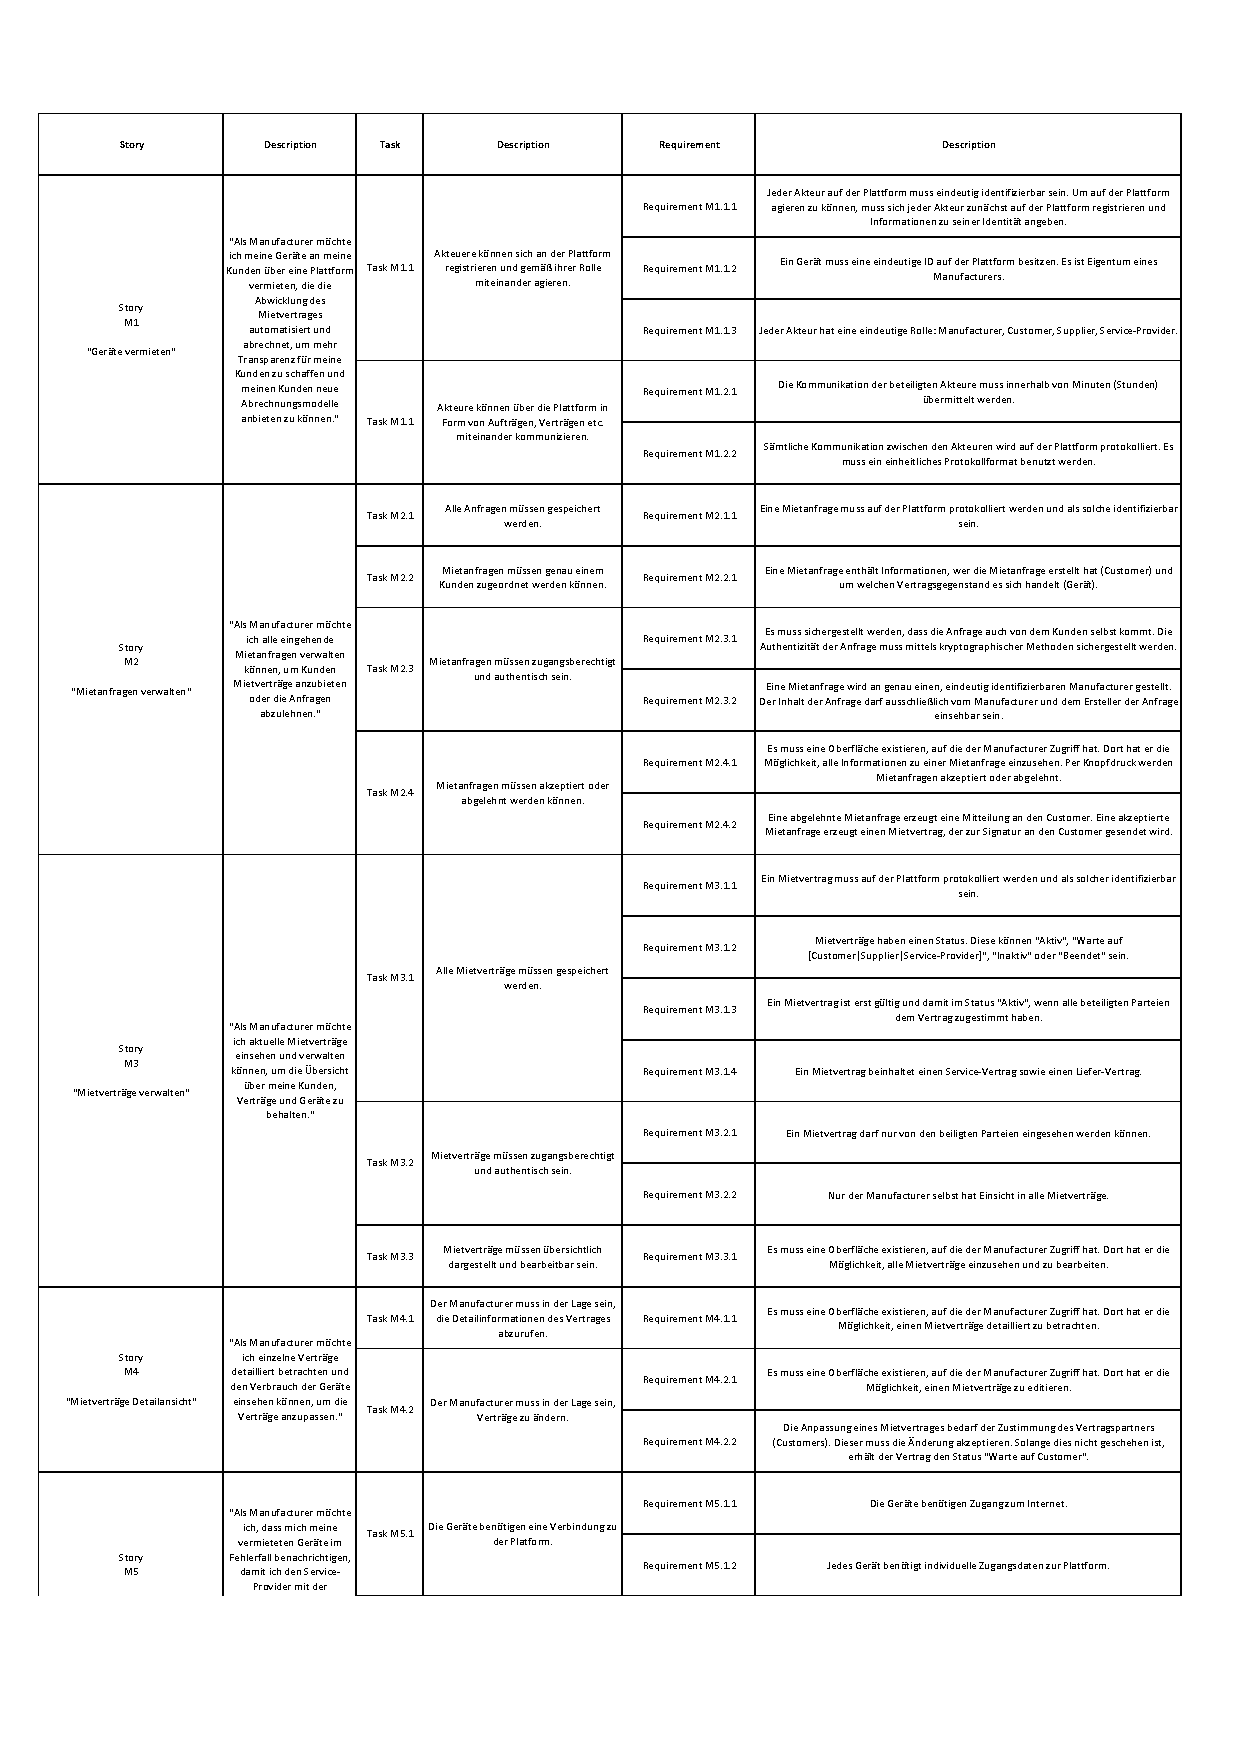
\includepdf[pages=-]{gfx/Requirements_v1.pdf}
\end{center}
\end{adjustwidth}
\newpage


\chapter{Appendix: DLT-Marktübersicht}
\label{ch:appendix:dlts}

\begin{table}[]
\caption[IOT-Relevanz]{IOT-Relevanz, \url{https://cryptoslate.com/cryptos/iot} (Stand: 30.12.19 10:00 Uhr)}
\label{tab:_iot}
\centering
\begin{tabular}{@{}lllllllll@{}}
\toprule
\textbf{Name} & \textbf{Blockchain} & \textbf{Marketcap} & \textbf{Price} & \textbf{Volume} \\ \midrule
IOTAMIOTA & \$456.91M & \$0.16438 & \$5,388,399 & -1.16\% \\
IoTeXIOTX & \$19.11M & \$0.00354 & \$1,873,820 & -0.78\% \\
WaltonchainWTC & \$15.29M & \$0.35410 & \$1,762,594 & -5.61\% \\
RobotinaROX & \$13.18M & \$0.04337 & \$128,840 & +0.06\% \\
IoT ChainITC & \$9M & \$0.10783 & \$1,769,855 & -1.07\% \\
INT ChainINT & \$6.58M & \$0.01732 & \$1,032,942 & +1.77\% \\
RuffRUFF & \$5.11M & \$0.00521 & \$904,692 & +1.24\% \\
XensorXSR & \$3.58M & \$0.01008 & \$5,971,333 & -38.27\% \\
ArtfinityAT & \$3.03M & \$0.02406 & \$8,018,680 & -0.54\% \\
SDChainSDA & \$2.23M & \$0.00149 & \$12,165 & -12.22\% \\ \bottomrule
\end{tabular}
\end{table}



\begin{table}[]
\caption[Blocktivity]{Blocktivity, \url{https://blocktivity.info/} (Stand: 31.12.19 10:00 Uhr)}
\label{tab:_blocktivity}
\centering
\begin{tabular}{@{}lllllll@{}}
\toprule
\textbf{Name} & \textbf{Activity} & \textbf{Average (7d)} & \textbf{Record} & \textbf{Market Cap} & \textbf{AVI} \\ \midrule
EOS & 56,068,563Op & 52,464,432Op & 74,568,958Op & \$ 2.6 B & 6,837 \\
TLOS & 6,973,820Op & 6,886,382Op & 32,217,207Op & \$ 0.013 B & 175,396 \\
IOST & 1,542,547Op & 955,269Op & 1,651,712Op & \$ 0.061 B & 7,893 \\
XLM & 1,186,730Op & 1,277,089Op & 1,391,425Op & \$ 0.923 B & 404 \\
KIN & 1,160,424Op & 1,080,820Op & 5,258,216Op & \$ 0.004 B & 87,014 \\
TRX & 1,069,788Op & 1,148,209Op & 5,306,869Op & \$ 0.930 B & 362 \\
STEEM & 996,699Op & 996,699Op & 2,522,380Op & \$ 0.047 B & 6,671 \\
NANO & 592,744Op & 663,973Op & 1,007,236Op & \$ 0.090 B & 2,072 \\
ETH & 509,869Op & 566,058Op & 1,372,918Op & \$ 15 B & 11 \\
BSV & 443,946Op & 479,188Op & 900,436Op & \$ 1.8 B & 77 \\ \bottomrule
\end{tabular}
\end{table}



\begin{table}[]
\caption[Coincodecap]{Coincodecap, \url{https://coincodecap.com/coins} (Stand: 29.12.2019 14:30 Uhr)}
\label{tab:_coincodecap}
\centering
\begin{tabular}{@{}lllllllll@{}}
\toprule
\textbf{Name} & \textbf{Commits} & \textbf{Stars} & \textbf{Releases} & \textbf{\begin{tabular}[c]{@{}l@{}}Active\\   Authors\end{tabular}} & \textbf{Languages} \\ \midrule
Ethereum (ETH) & 10270 & 89285 & 97 & 524 & 14 \\
LBRY Credits (LBC) & 13999 & 10826 & 261 & 170 & 12 \\
Lisk (LSK) & 31697 & 7874 & 92 & 69 & 5 \\
Cosmos (ATOM) & 4890 & 9198 & 98 & 284 & 13 \\
Stellar (XLM) & 5281 & 6627 & 174 & 168 & 14 \\
WAVES (WAVES) & 18262 & 2367 & 32 & 163 & 17 \\
EOS (EOS) & 12230 & 17557 & 81 & 134 & 16 \\
IOTA (MIOTA) & 10316 & 7759 & 79 & 145 & 15 \\ \bottomrule
\end{tabular}
\end{table}



\begin{table}[]
\caption[Github Commits past 12 months]{Github Commits past 12 months, \url{https://www.cryptomiso.com/} (Stand: 29.12.2019 14:30 Uhr)}
\label{tab:_cryptomiso}
\centering
\begin{tabular}{@{}llllllll@{}}
\toprule
\textbf{Crypto} & \textbf{Commits} & \textbf{Contributors} & \textbf{Watchers} \\ \midrule
Bitcoin & 1921 & 100 & 41697 \\
Ethereum & 851 & 100 & 25146 \\
EOS & 1783 & 100 & 10764 \\
Tron & 2796 & 99 & 2325 \\
Monero & 844 & 100 & 4177 \\
Zcash & 475 & 100 & 4110 \\
Lisk & 6586 & 62 & 2685 \\
Syscoin & 2388 & 100 & 108 \\
Particl & 2146 & 100 & 91 \\
BitcoinCash & 1277 & 100 & 872 \\ \bottomrule
\end{tabular}
\end{table}



\begin{table}[]
\caption[Blockchain Projekte in großen internationalen Unternehmen (Teil 1)]{Blockchain Projekte in großen internationalen Unternehmen (Teil 1), \cite{forbes2018} (Stand: 29.12.19 17:00 Uhr)}
\label{tab:_forbes}
\centering
\begin{tabular}{@{}lll@{}}
\toprule
\textbf{\begin{tabular}[c]{@{}l@{}}Hyperledger\\   Fabric\end{tabular}} & \textbf{Ethereum} & \textbf{Corda} \\ \midrule
Allianz SE & Amazon & Allianz SE \\
Amazon & Anheuser-Busch InBev & Anheuser-Busch InBev \\
BBVA & BBVA & BBVA \\
BNP Paribas & BNP Paribas & BNP Paribas \\
Broadridge & BP PLC & HPE \\
Comcast & Ciox Health & ING \\
HPE & Citigroup & Intel \\
ING & Coinbase & Maersk \\
Intel & Comcast & Microsoft \\
Microsoft & Fidelity & Nasdaq \\
Nasdaq & Foxconn & PNC \\
Northern Trust & Google & Siemens \\
PNC & HPE & State Farm \\
Santander & HTC & UBS \\
SAP SE & Intel &  \\
Seagate Technology & Microsoft &  \\
Siemens & Northern Trust &  \\
State Farm & Overstock &  \\
UBS & Samsung &  \\
Visa & Siemens &  \\
Walmart & UBS &  \\ \bottomrule
\end{tabular}
\end{table}

\begin{table}[]
\caption[Blockchain Projekte in großen internationalen Unternehmen (Teil 2)]{Blockchain Projekte in großen internationalen Unternehmen (Teil 2), \cite{forbes2018} (Stand: 29.12.19 17:00 Uhr)}
\label{tab:_forbes2}
\centering
\begin{tabular}{@{}llll@{}}
\toprule
\textbf{Quorum} & \textbf{Bitcoin} & \textbf{\begin{tabular}[c]{@{}l@{}}Hyperledger\\ Sawtooth\end{tabular}} & \textbf{Ripple} \\ \midrule
BP PLC & Bitfury & Cargill & Coinbase \\
Broadridge & Coinbase & CVS Health & PNC \\
Comcast & Comcast & Intel & Santander \\
HPE & Fidelity &  &  \\
ING & Google &  &  \\
JPMorgan Chase & HTC &  &  \\
Microsoft & Overstock &  &  \\
SAP SE &  &  &  \\
State Farm &  &  &  \\
UBS &  &  &  \\ \bottomrule
\end{tabular}
\end{table}
\newpage


\chapter{Appendix: DLT-Auswahl}
\label{ch:appendix:dlt_selection}
% Please add the following required packages to your document preamble:
% \usepackage{booktabs}
\begin{table}[htbp]
\caption{Erstauswahl von DLT-Lösungen}
\label{tab:dlt_preselection}
\begin{tabular}{lccccr}
\hline
\textbf{} & \textbf{\begin{tabular}[c]{@{}c@{}}Business\\ Relevance\end{tabular}} & \textbf{\begin{tabular}[c]{@{}c@{}}Github\\ Activity\end{tabular}} & \textbf{\begin{tabular}[c]{@{}c@{}}Blockchain\\ Activity\end{tabular}} & \textbf{IOT} & \textbf{TOTAL} \\
 & 2 & 1 & 1 & 1,5 &  \\ \hline
Bitcoin & x & x &  &  & 3 \\
Bitcoin SV &  &  & x &  & 1 \\
BitcoinCash & x & x &  &  & 3 \\
Cardano &  & x &  &  & 1 \\
Corda & x &  &  &  & 2 \\
Cosmos &  & x &  &  & 1 \\
EOS &  & x & x &  & 2 \\
Ethereum & x & x & x &  & 4 \\
Hyperledger & x &  &  &  & 2 \\
INT Chain &  &  &  & x & 1,5 \\
IOST &  &  & x &  & 1 \\
IoT Chain &  &  &  & x & 1,5 \\
IOTA &  & x &  & x & 2,5 \\
KIN &  &  & x &  & 1 \\
LBRY Credits &  & x &  &  & 1 \\
Lisk &  & x &  &  & 1 \\
Monero &  & x &  &  & 1 \\
Nano &  &  & x &  & 1 \\
Particl &  & x &  &  & 1 \\
Quorum & x &  &  &  & 2 \\
Ripple & x &  &  &  & 2 \\
Ruff &  &  &  & x & 1,5 \\
SDChain &  &  &  & x & 1,5 \\
Steem &  &  & x &  & 1 \\
Stellar &  & x & x &  & 2 \\
Syscoin &  & x &  &  & 1 \\
Telos &  &  & x &  & 1 \\
Tron &  & x & x &  & 2 \\
WAVES &  & x &  &  & 1 \\
Zcash &  & x &  &  & 1 \\ \hline
\end{tabular}
\end{table}


\newpage

\chapter{Appendix: Umsetzung}
\label{ch:appendix:implementation}

\section{Benutzerinteraktionen}
\label{sec:appendix:implementation:interactions}
Der vorliegende IOT-Anwendungsfall beinhaltet verschiedene Benutzerinteraktionen, die anhand der folgenden \ac{UML}-Sequenzdiagramme dargestellt und erläutert werden.\\

\begin{figure}[h]
 \centering
 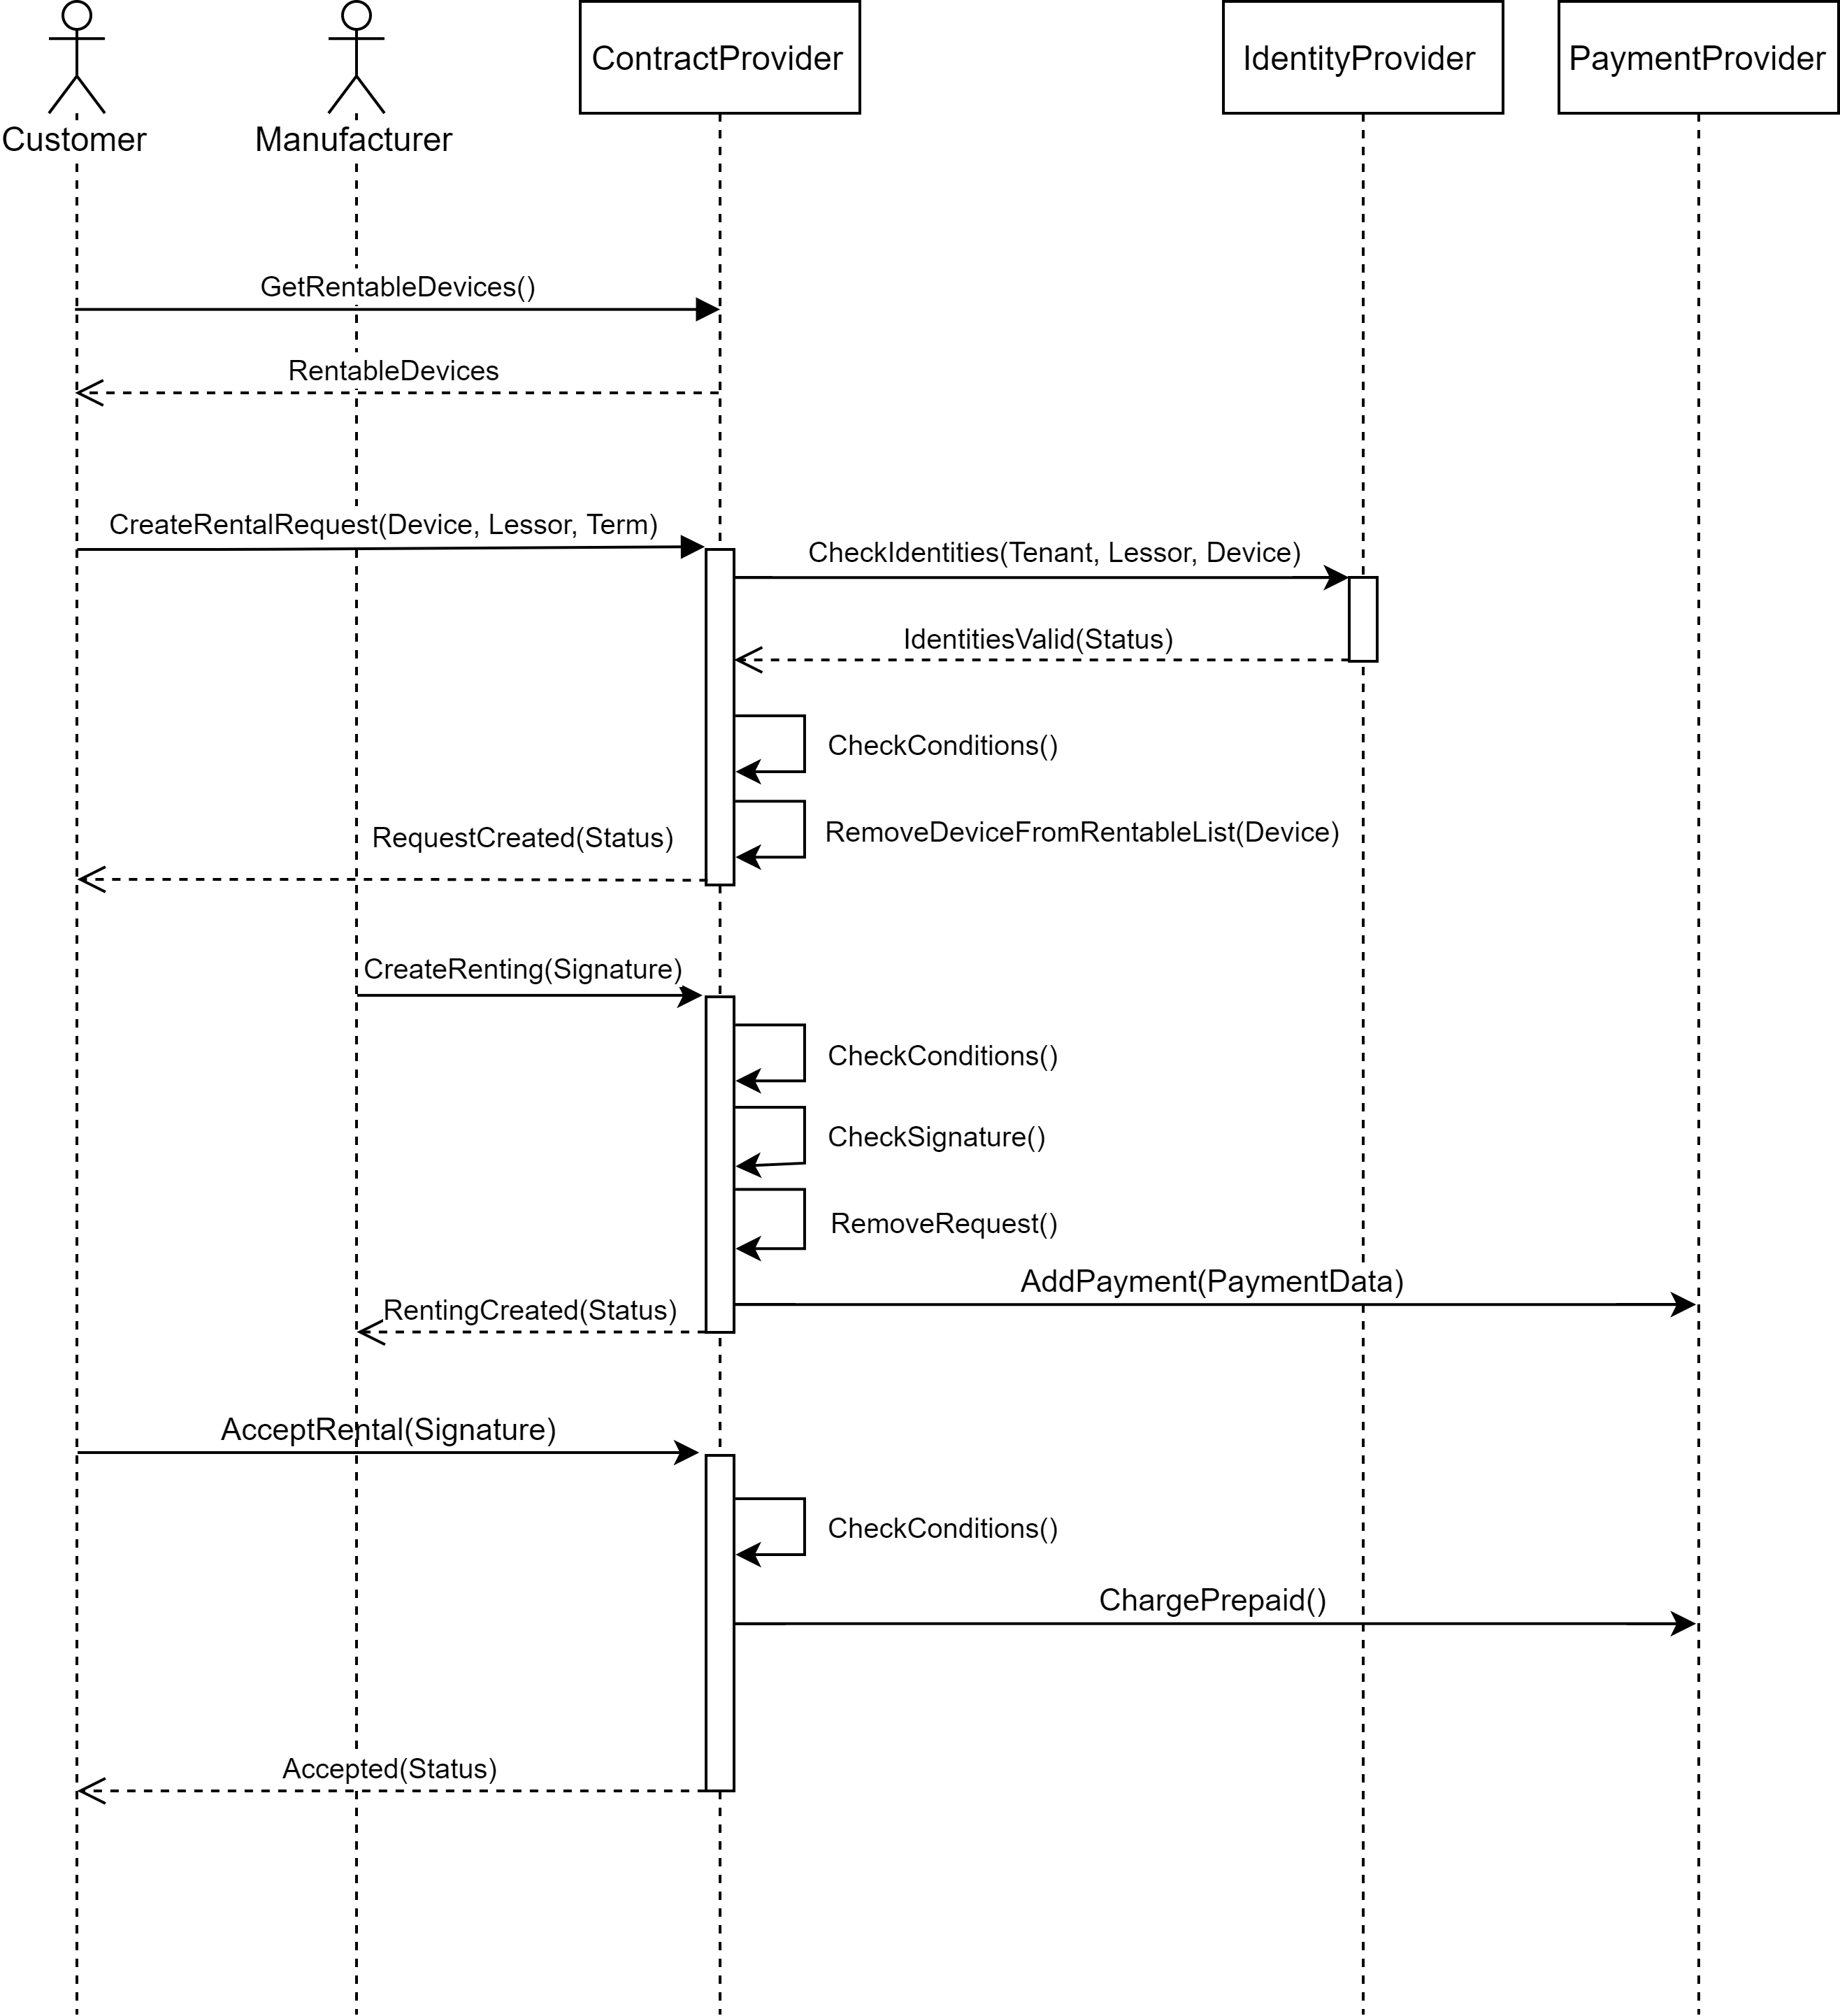
\includegraphics[width=1.0\textwidth]{gfx/UML_Seq-ContractCreation.png}
 \caption{UML-Sequenzdiagramm zur Vertragserzeugung}
 \label{fig:chapter07:creation}
\end{figure}
Die Vertragserzeugung kann grob in drei Schritte untergliedert werden und wird initial durch den Benutzer ausgelöst. Im ersten Schritt hat der Benutzer über das Web-Frontend Zugriff auf die verfügbaren Miet-Geräte. Aus diesen Geräten wählt er eines aus und erzeugt eine Mietanfrage, die per API-Call an den RentalProvider Smart-Contract gesendet wird. Dieser führt Überprüfungen aus wie die Kontrolle der Identitäten, Inhalte der Mietanfrage und markiert nach erfolgreicher Prüfung das Gerät als reserviert, sodass es kein anderer Benutzer anmieten kann. Der zweite Schritt wird durch den Hersteller des Gerätes gestartet: Dieser kann die Mietanfrage prüfen und anschließend akzeptieren, indem er einen von ihm signierten Mietvertrag an den RentalProvider sendet. Lehnt er die Anfrage ab, so wird die Mietanfrage gelöscht und das Gerät als wieder verfügbar markiert. Stimmen die Daten des Mietvertrages und ist die Signatur valide, wird der Mietvertrag gespeichert und ein dazugehöriger Payment-Channel eröffnet. Der letzte Schritt wird wieder durch den Benutzer ausgeführt: Der vom Hersteller erzeugte Mietvertrag kann geprüft und die Vertragsbedingungen (Vertragslaufzeiten, Kosten, etc.) eingesehen werden. Akzeptiert der Benutzer den Mietvertrag durch seine Signatur, wechselt dieser in den Status aktiv. Gleichzeitig transferiert der Benutzer ein Startguthaben von seinem Wallet auf den zum Mietvertrag angelegten Payment-Channel. Die Benutzung kann anschließend sofort erfolgen.

\begin{figure}[h]
 \centering
 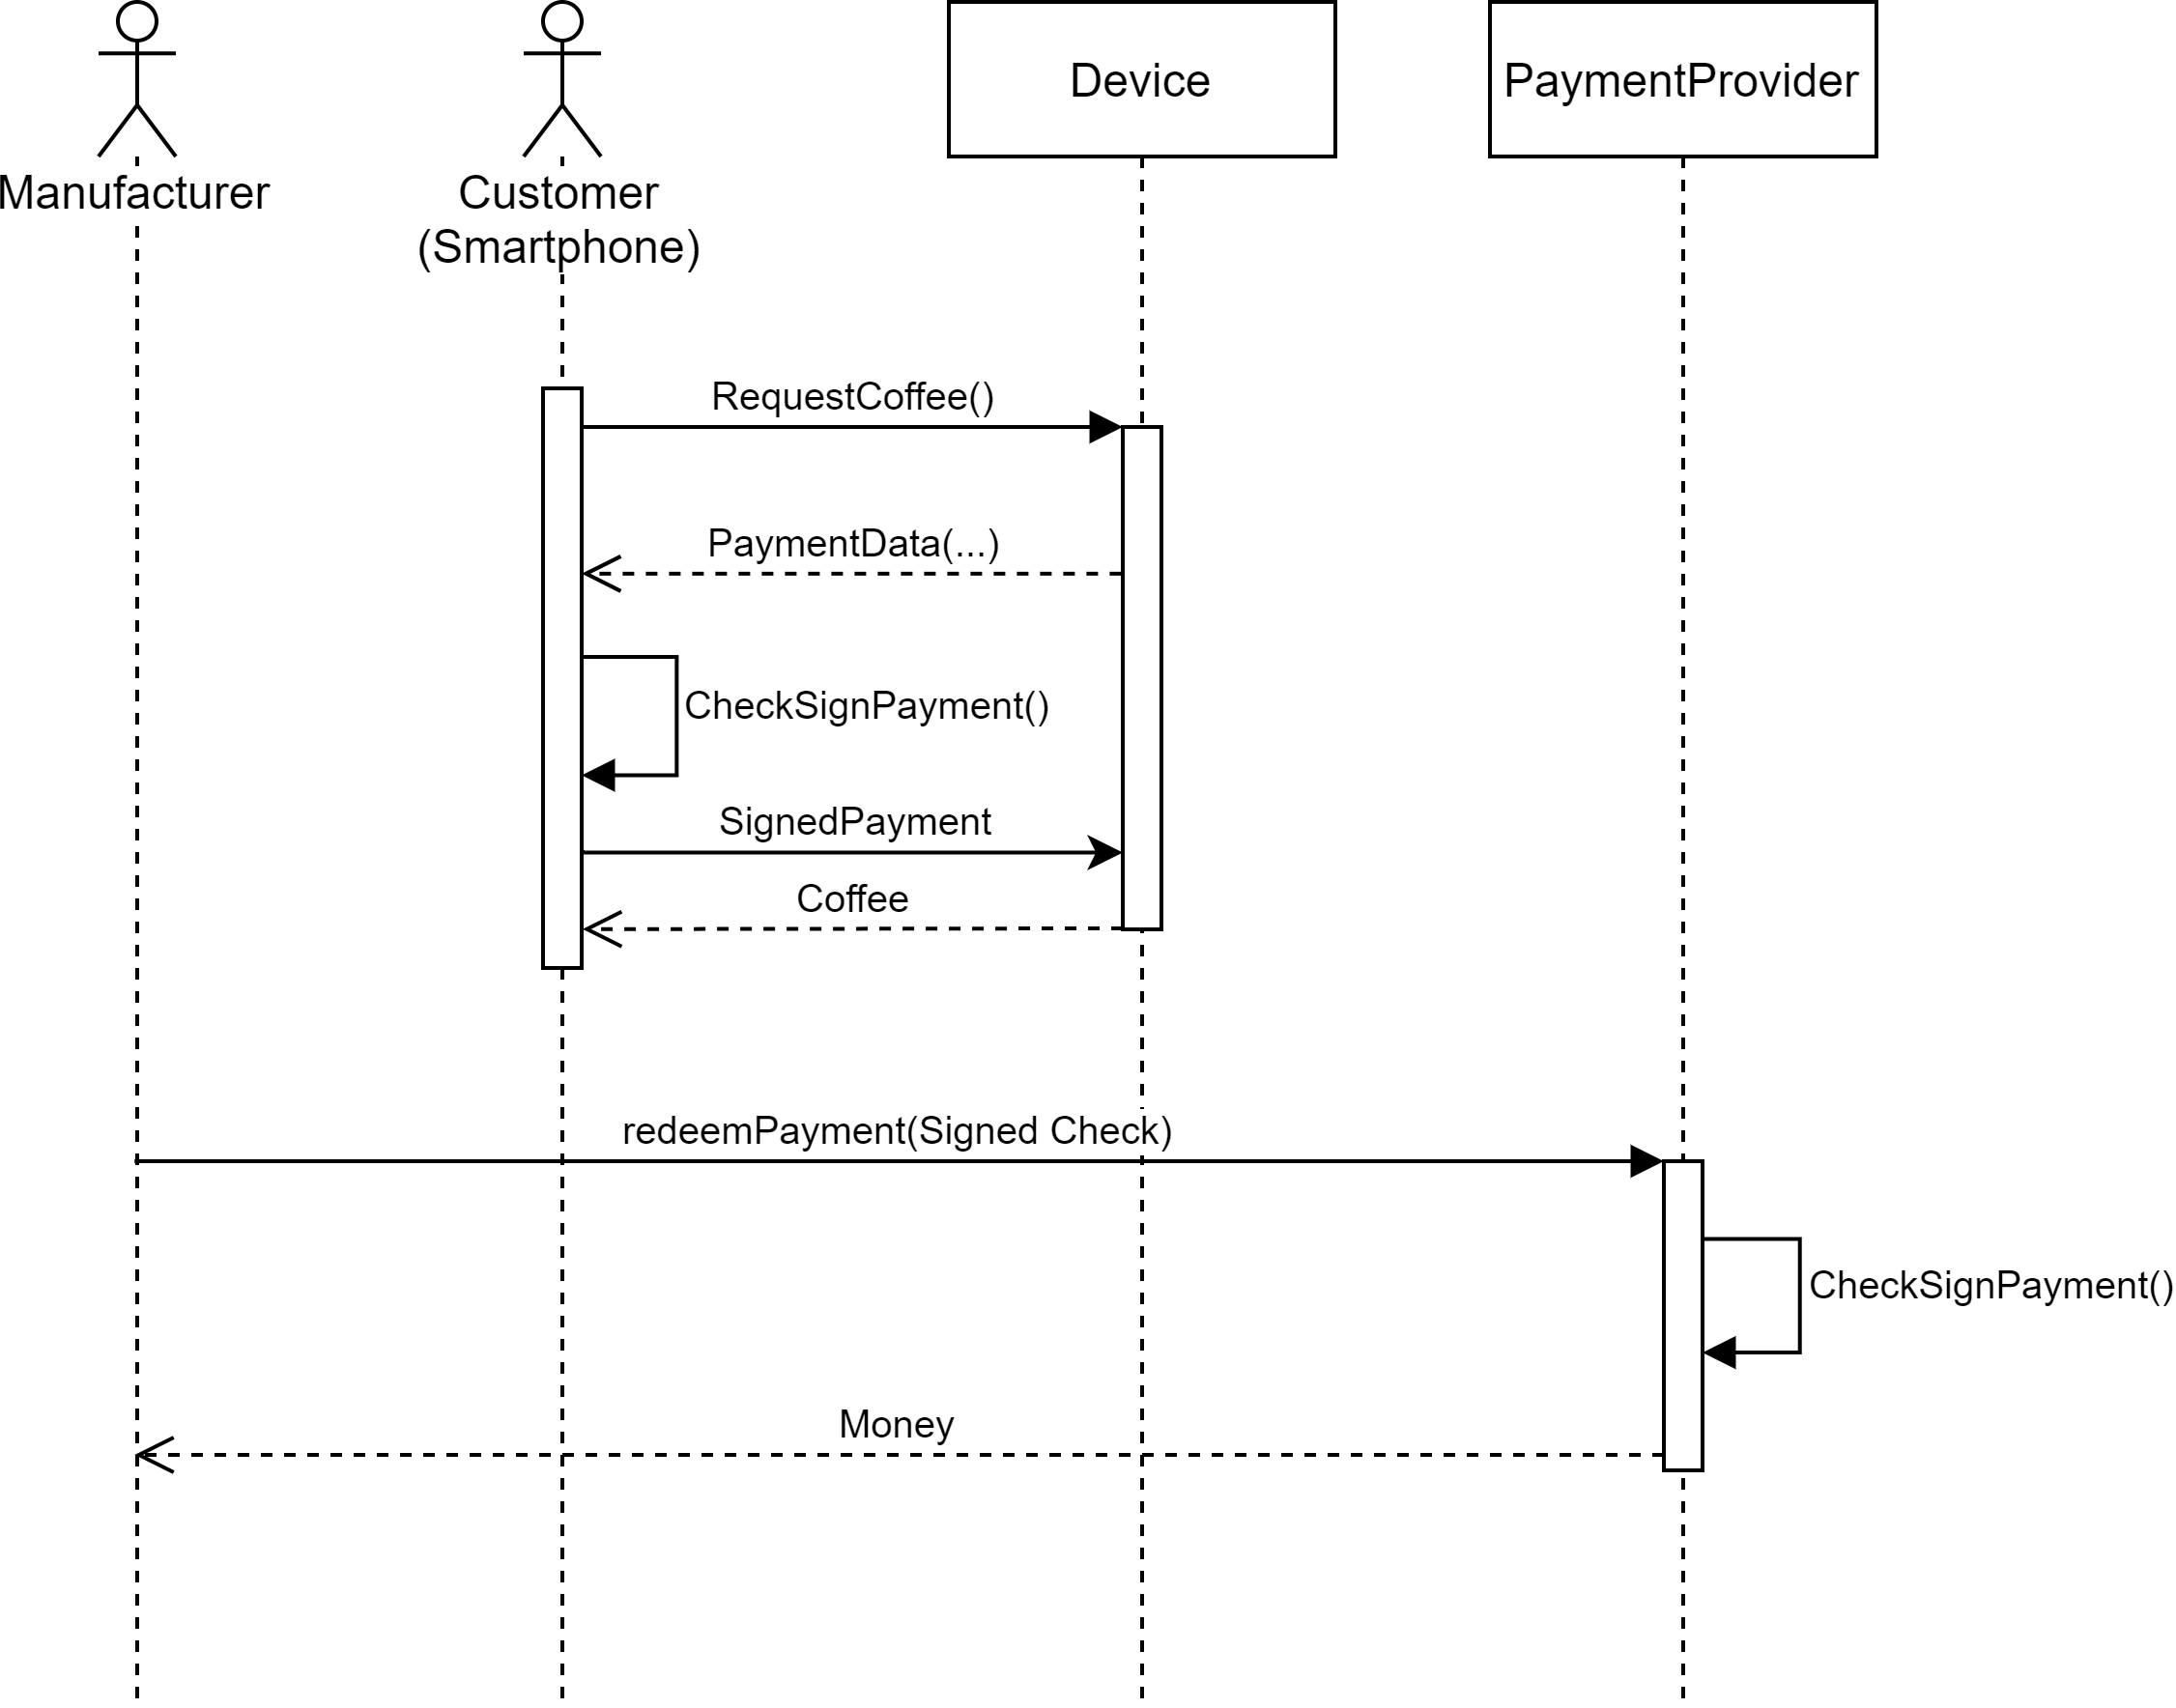
\includegraphics[width=1.0\textwidth]{gfx/UML_Seq-Usage.png}
 \caption{UML-Sequenzdiagramm zur Zahlungsabwicklung}
 \label{fig:chapter07:usage}
\end{figure}

Ein aktiver Mietvertrag ist Voraussetzung für die erfolgreiche Benutzung der Kaffeemaschine, da ansonsten kein Kaffee serviert wird. Fragt der Benutzer mittels Knopfdruck eine Tasse Kaffee an, erzeugt die Maschine eine Quittung, die bestätigt, dass der Kunde in einem festgelegten Zeitraum\footnote{Beginn des Zeitraums ist zu anfangs der Vertragsbeginn; wurde bereits eine Bezahlung durch Schließen des Payment-Channels eingelöst, so wird der Startzeitpunkt der folgenden Quittung auf den Zeitpunkt des Schließens gesetzt.} eine bestimmte Anzahl Kaffees zu einem festgelegten Preis konsumiert hat. Diese Quittung wird mittels \ac{NFC} an das Smartphone des Benutzers gesendet, dort überprüft, mittels des Private-Keys signiert und anschließend über die gleiche Schnittstelle zurückgesendet. Ist die Signatur korrekt, serviert die Maschine die vereinbarte Menge Kaffee. Alle zahlungsrelevanten Informationen liegen zu diesem Zeitpunkt lokal auf der Maschine. Wird die Maschine kompromittiert oder führt ein interner Fehler zum Verlust der signierten Quittung, besteht keine Möglichkeit, die Zahlungen geltend zu machen. Sofern eine Konnektivität zum Internet besteht, können verschiedene Mechanismen implementiert werden, um die Zahlungsinformationen zu schützen. Der eigentliche Bezahlvorgang, also das Transferieren von Geldern, erfolgt durch das Übertragen der signierten Quittung an den PaymentProvider Smart-Contract. Dieser überprüft die Quittung sowie die Signatur des Benutzers und transferiert die quittierte Menge Geld (in diesem Fall Ether) an den Hersteller. In der vorliegenden Implementierung wird die Quittung durch die Maschine im Namen des Herstellers eingelöst. Diese Umsetzung ist nicht optimal, da der Private-Key des Herstellers damit lokal auf der Maschine vorliegen muss, wurde allerdings aufgrund der Einfachheit so umgesetzt. Ein Optimierungsansatz hierzu wird im Kapitel \ref{ch:perspective} vorgestellt. Der Zeitpunkt, wann eine Maschine eine Quittung einlösen sollte, wird in Abschnitt \ref{subsec:implementation:requirements:async} genauer betrachtet.

\newpage

\section{Deployment}
\label{sec:appendix:implementation:deployment}

\begin{table}[h]
  \caption{Adressen der Smart-Contracts auf dem öffentlichen Ropsten Testnet}
\label{tab:ropsten}
\begin{tabular}{@{}cl@{}}
\toprule
\textbf{Smart-Contract} & \multicolumn{1}{c}{\textbf{Ropsten-Adresse}} \\ \midrule
Rental-Provider & 0x851ED36AC125a04A7384d485D0E5b710d1e8AB96 \\
Identity-Provider & 0xA17351BfA16dAE1FD285e11AcC00882Eb459C7cb \\
Payment-Provider & 0x182B60f63AE760B137D479E00e823b0C027736eE \\ \bottomrule
\end{tabular}

\end{table}

\newpage

\section{Kostenevaluation}
\label{sec:appendix:implementation:costs}

% Please add the following required packages to your document preamble:
% \usepackage{booktabs}
\begin{table}[h]
\caption{Basisdaten für Kostenkalkulationen, inklusive der Annahmen}
\label{tab:calc1}
\begin{adjustwidth}{-.5in}{-.5in}
\begin{center}
\begin{tabular}{@{}llll@{}}
\toprule
\multicolumn{1}{c}{\textbf{Beschreibung}} & \multicolumn{1}{c}{\textbf{Anzahl}} & \multicolumn{1}{c}{\textbf{Einheit}} & \multicolumn{1}{c}{\textbf{Annahme}} \\ \midrule
GAS-Price & 5 & GWEI &  \\
ETH-Kurs & 196,04 & Euro &  \\
Anzahl Kaffeemaschinen & 10.000 & Maschinen & x \\
Mitarbeiter pro Kaffeemaschine & 40 & Mitarbeiter & x \\
Mitarbeiter gesamt & 400.000 & Mitarbeiter &  \\
Liter Kaffee pro Jahr pro Person & 164 & Liter &  \\
Tassen Kaffee (0,2l) pro Jahr & 820 & Tassen &  \\
Arbeitstage (abzgl. 30 Tage Urlaub) & 230 & Tage &  \\
Tassen Kaffee (0,2l) pro Tag & 2,24 & Tassen &  \\
Prepaid-Guthaben ausreichend für & 5 & Tage (Arbeitswoche) &  \\
Preis pro Tasse Kaffee & 0,25 & Euro & x \\
Umsatzvolumen pro Maschine und Woche & 157,69 &  &  \\
\begin{tabular}[c]{@{}l@{}}Prepaid Guthaben pro Maschine\\   aufladen\end{tabular} & 200 & Euro & \begin{tabular}[c]{@{}l@{}}x\\ (inkl. Puffer)\end{tabular} \\
Gesamtumsatz (jährlich) & 82.000.000 & Euro &  \\
Gesamtumsatz pro Maschine (jährlich) & 8.200 & Euro &  \\ \bottomrule
\end{tabular}
\end{center}
\end{adjustwidth}
\end{table}


% Please add the following required packages to your document preamble:
% \usepackage{booktabs}
\begin{table}[h]
\caption{Einzelkosten der Transaktion}
\label{tab:calc2}
\begin{adjustwidth}{-.5in}{-.5in}
\begin{center}
\begin{tabular}{@{}llllll@{}}
\toprule
\multicolumn{1}{c}{\textbf{Sender}} & \multicolumn{1}{c}{\textbf{Transaktion}} & \multicolumn{1}{c}{\textbf{GAS}} & \multicolumn{1}{c}{\textbf{WEI}} & \multicolumn{1}{c}{\textbf{ETH}} & \multicolumn{1}{c}{\textbf{Euro}} \\ \midrule
Hersteller & Vertrag erstellen & 426.609 & 2.133.045 & 0,002133 & 0,42 \\
Hersteller & Quittung einlösen & 157.927 & 789.635 & 0,00079 & 0,15 \\ \midrule
Kunde & Vertrag anfragen & 197.964 & 989.820 & 0,00099 & 0,19 \\
Kunde & Vertrag annehmen & 162.743 & 813.715 & 0,000814 & 0,16 \\
Kunde & Prepaid aufladen & 28.805 & 144.025 & 0,000144 & 0,03 \\ \bottomrule
\end{tabular}
\end{center}
\end{adjustwidth}
\end{table}


% Please add the following required packages to your document preamble:
% \usepackage{booktabs}
\begin{table}[h]
\caption{Gesamtkosten (einmalig und jährlich) der Transaktionen aus Nutzer- und Herstellersicht}
\label{tab:calc3}
\begin{adjustwidth}{-1.5in}{-1.5in}
\begin{center}
  \begin{tabular}{@{}lllllll@{}}
  \toprule
  \multicolumn{1}{c}{\textbf{Tx.}} & \multicolumn{1}{c}{\textbf{\begin{tabular}[c]{@{}c@{}}Tx. pro\\ Maschine\\     (einmalig)\end{tabular}}} & \multicolumn{1}{c}{\textbf{\begin{tabular}[c]{@{}c@{}}Tx.-Kosten\\ pro  Maschine\\     (einmalig)\end{tabular}}} & \multicolumn{1}{c}{\textbf{\begin{tabular}[c]{@{}c@{}}Tx.-Kosten\\ aller  Maschinen\\     (einmalig)\end{tabular}}} & \multicolumn{1}{c}{\textbf{\begin{tabular}[c]{@{}c@{}}Tx. pro\\ Maschine\\     (jährlich)\end{tabular}}} & \multicolumn{1}{c}{\textbf{\begin{tabular}[c]{@{}c@{}}Tx.-Kosten\\ pro  Maschine\\     (jährlich)\end{tabular}}} & \multicolumn{1}{c}{\textbf{\begin{tabular}[c]{@{}c@{}}Tx.-Kosten\\ aller  Maschinen\\     (jährlich)\end{tabular}}} \\
  \textit{} & \textit{Anzahl} & \textit{Euro} & \textit{Euro} & \textit{Anzahl} & \textit{Euro} & \textit{Euro} \\ \midrule
  \begin{tabular}[c]{@{}l@{}}Vertrag\\ erstellen\end{tabular} & 1 & 0,42 & 4.200,00 & 0 & 0,00 & 0,00 \\
  \begin{tabular}[c]{@{}l@{}}Quittung\\ einlösen\end{tabular} & 0 & 0,00 & 0,00 & 52 & 7,80 & 78.000,00 \\ \midrule
  \begin{tabular}[c]{@{}l@{}}Vertrag\\ anfragen\end{tabular} & 1 & 0,19 & - & 0 & 0,00 & - \\
  \begin{tabular}[c]{@{}l@{}}Vertrag\\ annehmen\end{tabular} & 1 & 0,16 & - & 0 & 0,00 & - \\
  \begin{tabular}[c]{@{}l@{}}Prepaid\\ aufladen\end{tabular} & 0 & 0,00 & - & 41 & 1,23 & - \\ \bottomrule
  \end{tabular}
\end{center}
\end{adjustwidth}
\end{table}

\begin{figure}[h]
 \centering
 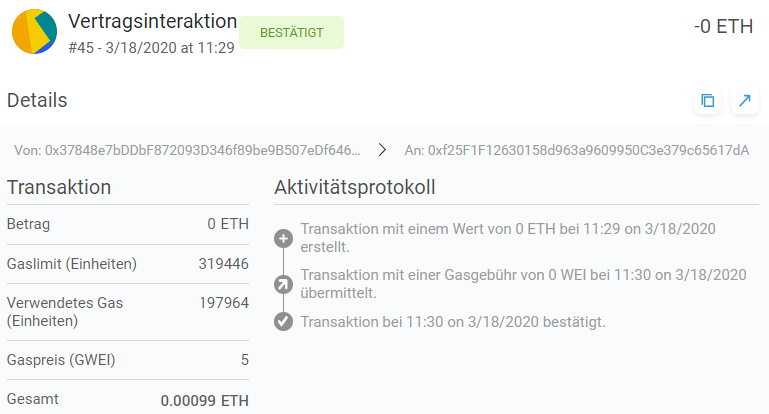
\includegraphics[width=1.0\textwidth]{gfx/screenshots/request_contract.PNG}
 \caption{Vertrag anfragen: Metamask Screenshot einer Transaktion}
 \label{fig:appendix:costs:request}
\end{figure}

\begin{figure}[h]
 \centering
 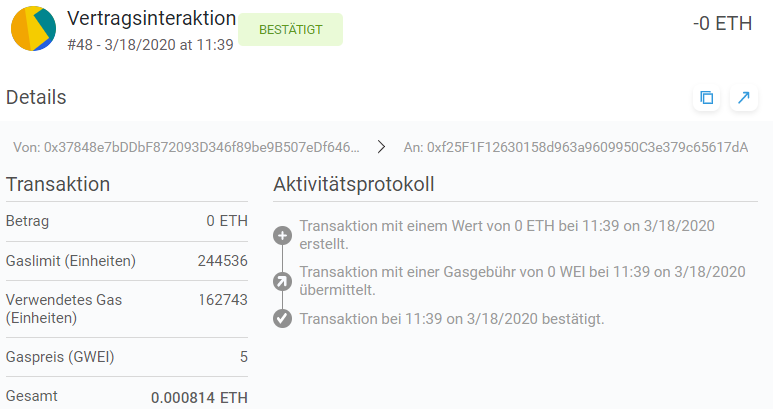
\includegraphics[width=1.0\textwidth]{gfx/screenshots/accept_contract.PNG}
 \caption{Vertrag akzeptieren: Metamask Screenshot einer Transaktion}
 \label{fig:appendix:costs:accept}
\end{figure}

\begin{figure}[h]
 \centering
 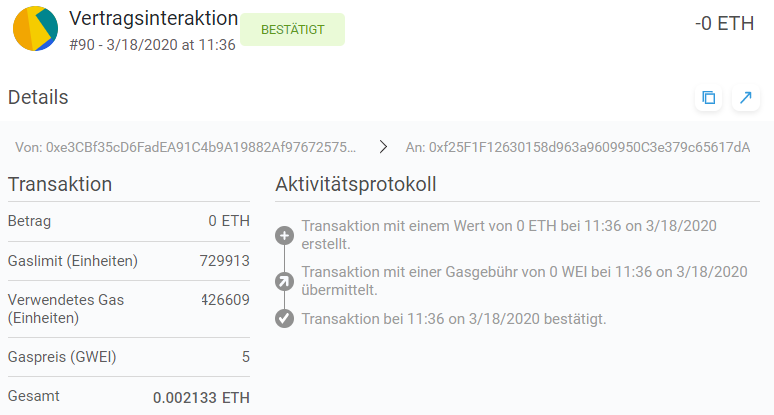
\includegraphics[width=1.0\textwidth]{gfx/screenshots/create_contract.PNG}
 \caption{Vertrag erzeugen: Metamask Screenshot einer Transaktion}
 \label{fig:appendix:costs:create}
\end{figure}

\begin{figure}[h]
 \centering
 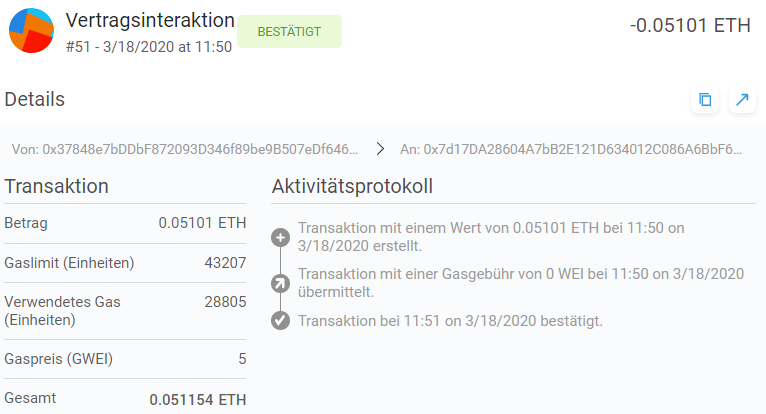
\includegraphics[width=1.0\textwidth]{gfx/screenshots/charge_contract.PNG}
 \caption{Prepaid Guthaben aufladen: Metamask Screenshot einer Transaktion}
 \label{fig:appendix:costs:charge}
\end{figure}

\begin{figure}[h]
 \centering
 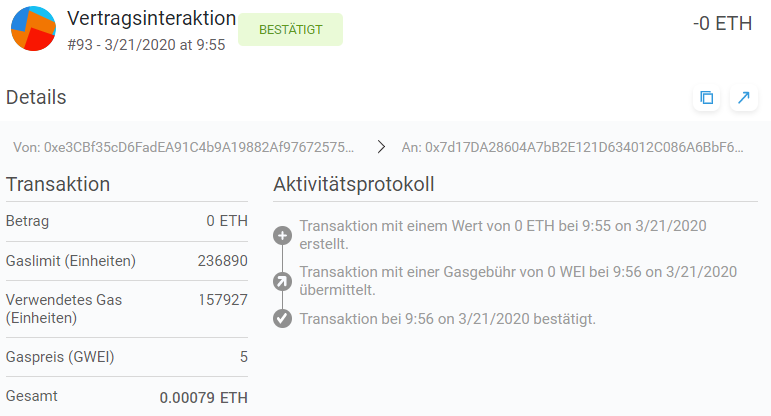
\includegraphics[width=1.0\textwidth]{gfx/screenshots/redeem.PNG}
 \caption{Quittung einlösen: Metamask Screenshot einer Transaktion}
 \label{fig:appendix:costs:reddeem}
\end{figure}


\clearpage

\section{UI}
\label{sec:appendix:implementation:ui}
\begin{figure}[h]
 \centering
 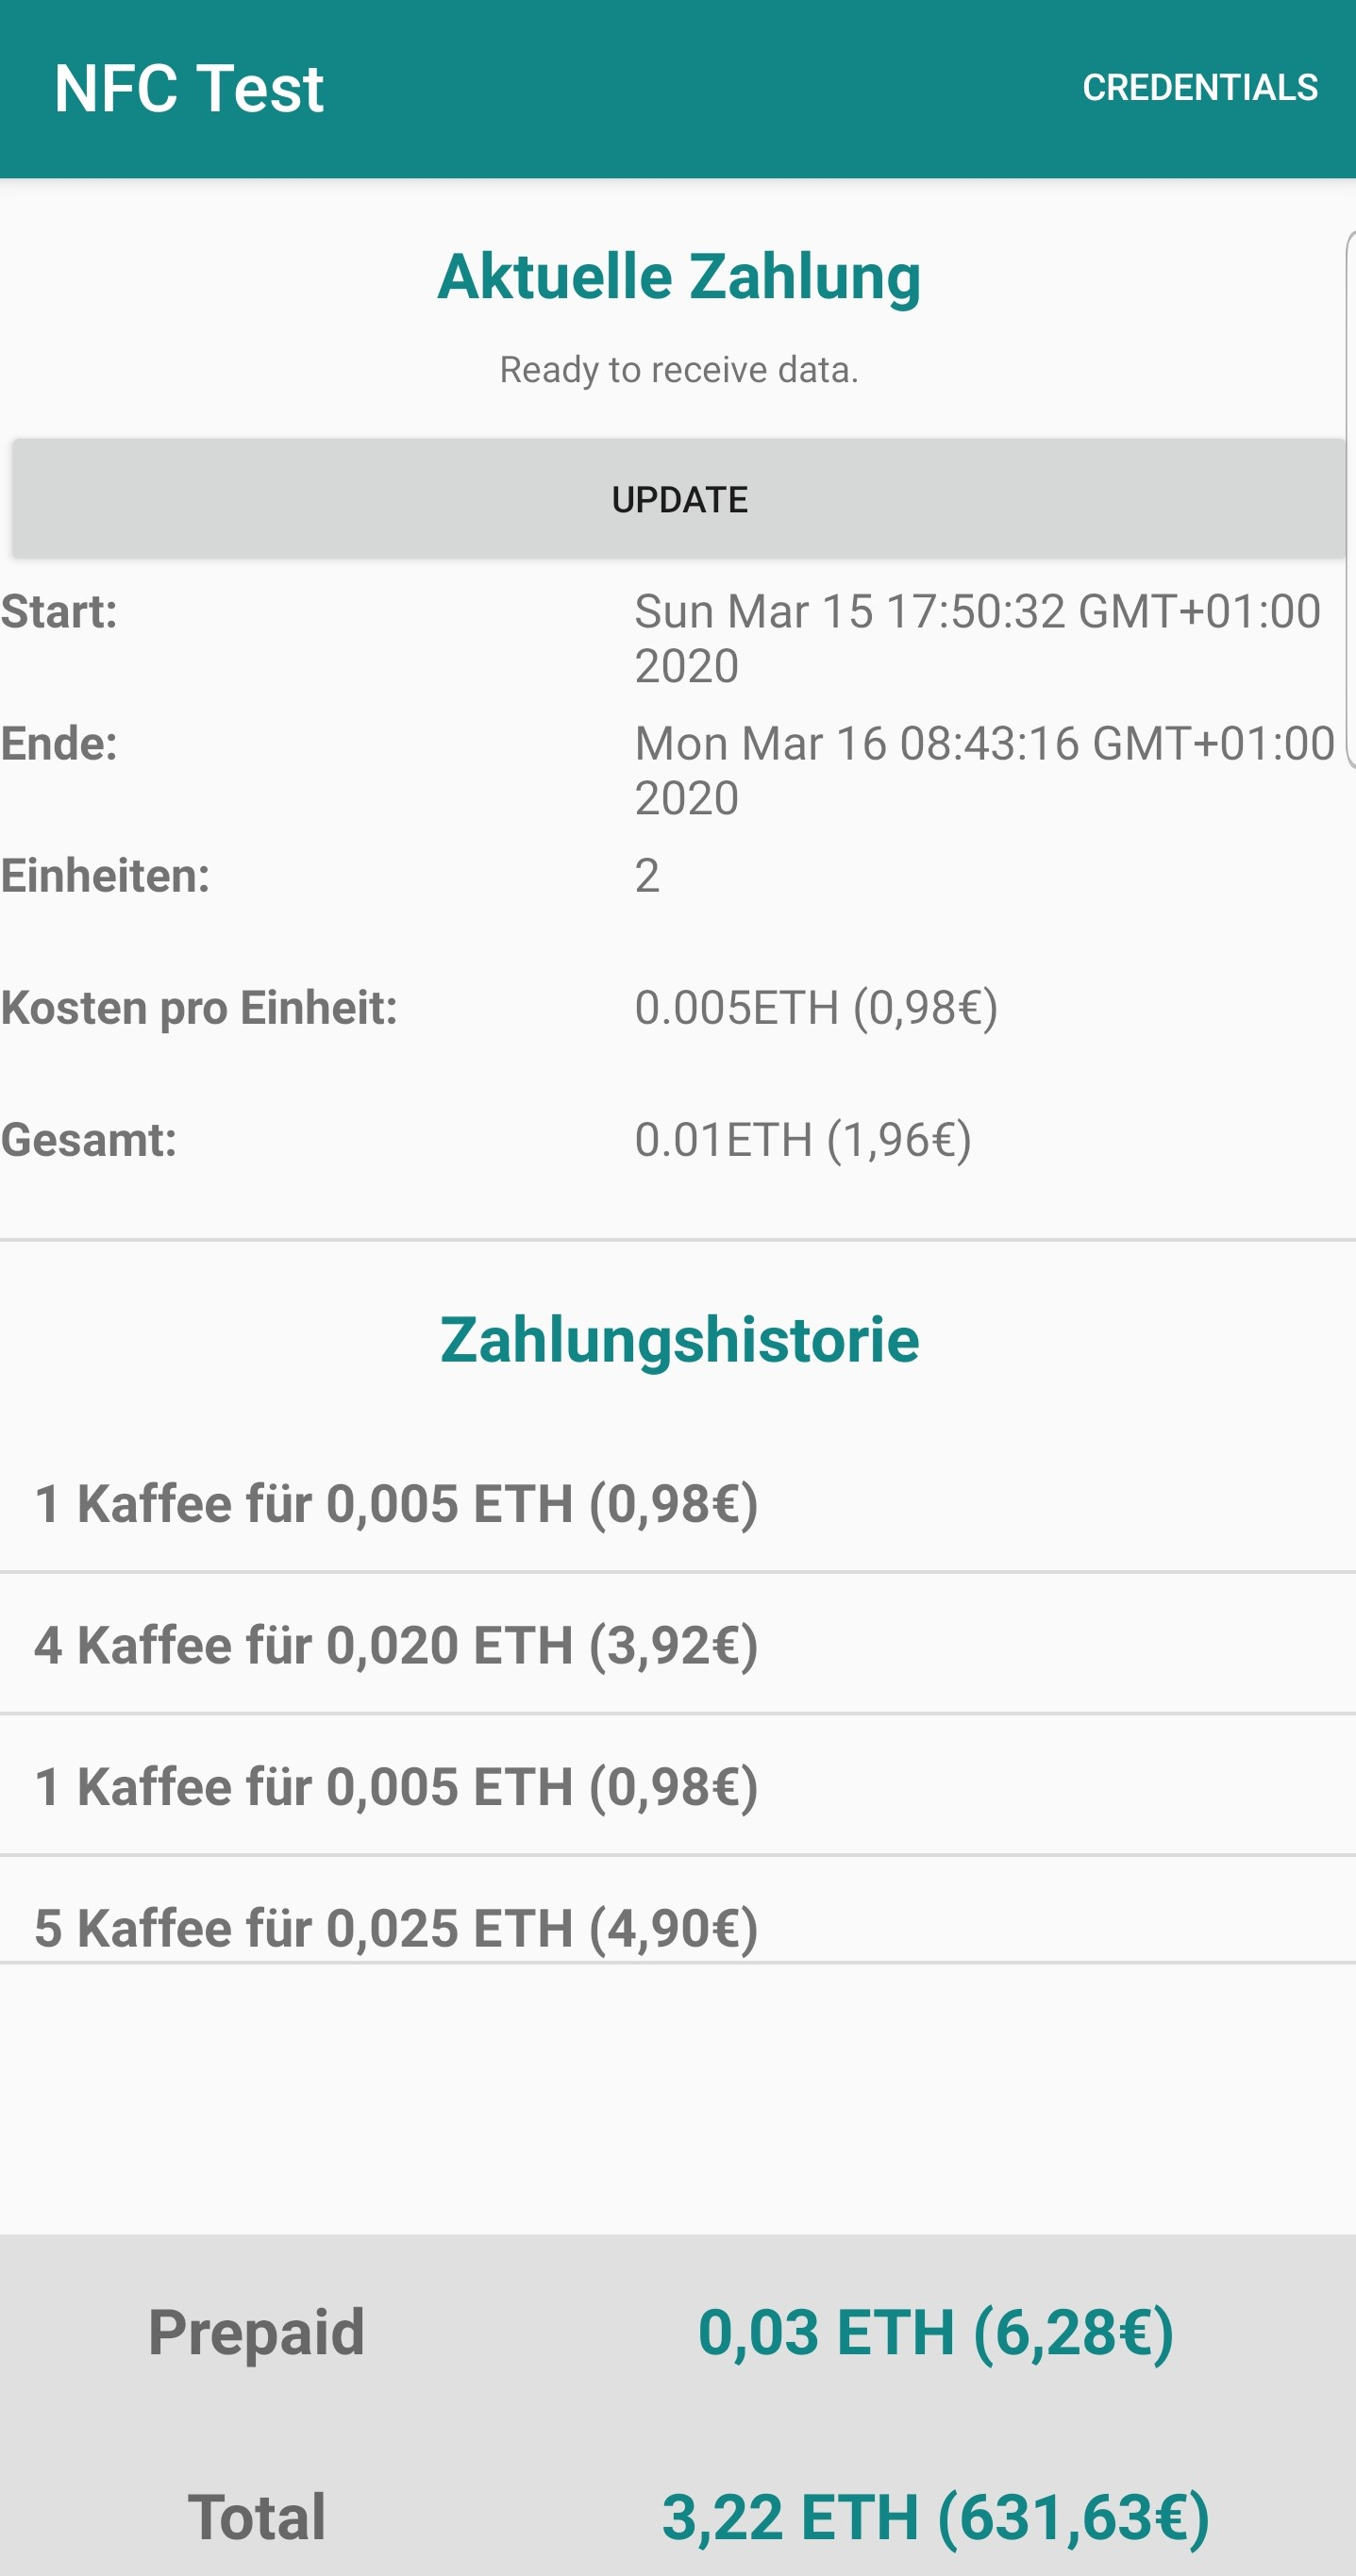
\includegraphics[width=0.4\textwidth]{gfx/screenshots/smartphone.jpg}
 \caption{Wallet-App auf Android-Basis}
 \label{fig:appendix:ui:smartphone}
\end{figure}
\newpage

\chapter{Appendix: Code}
\label{ch:appendix:code}

\lstinputlisting[caption=RentalProvider Smart-Contract]{gfx/code/RentalProvider.sol}
\lstinputlisting[caption=PaymentProvider Smart-Contract]{gfx/code/PaymentProvider.sol}
\lstinputlisting[caption=IdentityProvider Smart-Contract]{gfx/code/IdentityProvider.sol}
